\section{Introduction}\label{intro}
Developing machine learning-based applications is rarely a one-shot process requiring data pre-processing, iterating between model/feature design, analyzing the results, and evaluating the new model~\cite{sculley2014machine, krishnan2016hilda}.
While the community has made substantial progress in scalability and model specification~\cite{hellerstein2012madlib,tensor, kraska2013mlbase, crotty2014tupleware, keystone}, there are few tools to assist developers iterate, diagnose, and debug learning applications.


As deeper models (DNNs) become more popular, it is increasingly difficult to know what the model is learning and why the model mispredicts.
It can be unclear if a misprediction is due to inconsistencies in the training data, the model cannot represent the patterns in the data  (e.g., need more layers?), or since similar examples were simply not present in the training data.
For instance, consider designing prediction models for self-driving cars.  
Poor lighting conditions, street obstacles, and other issues could lead to highly noisy training data.
Furthermore, it is unlikely that the training data has collected data for every possible driving condition (e.g., during a once in five years storm).
For data scientists to effective design and debug learning applications, they need to be able to understand why a model made a certain prediction.

\begin{figure}
    \centering
    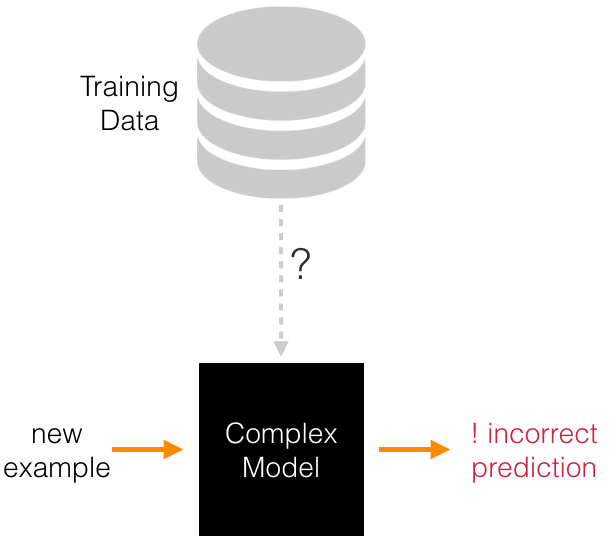
\includegraphics[width=0.35\columnwidth]{figures/teaser1.png}
    \hspace{2em}
    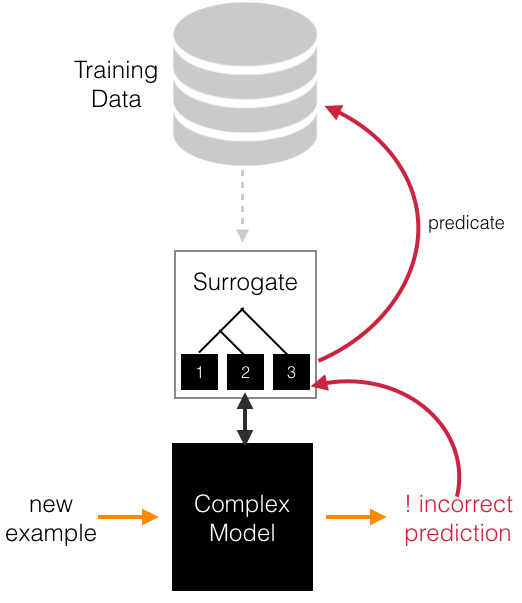
\includegraphics[width=0.35\columnwidth]{figures/teaser2.png}
    \caption{(Left) ML developers need to understand the relationship between training data and a model's predictions, i.e., how are similar points predicted in the training data. But effectively determining the size and range of this neighborhood is challenging in expressive models which can have very complex geometry. (Right) We propose an approximation technique that can represent a black-box model in terms of sub-models applied to feature-space partitions. The developer can quickly determine which data are related based on these partitions.}
    \label{fig:my_label}
\end{figure}

Two contrasting approaches have been pursued by the ML community: (1) use a simpler, more interpretable model (e.g., a decision tree) from the start, or (2) explain the behavior of a complex model using a simplified approximation~\cite{taylor2016alignment, lei2016rationalizing, ribeiro2016should}. This problem is extremely challenging.
Using a simpler model is often out of the question as modern ML models are complex for good reason---they map very high-dimensional images or documents to decisions.
In terms of explanations, one highly promising approach is to locally linearize a model in a small neighborhood to explain its behavior\cite{taylor2016alignment, lei2016rationalizing, ribeiro2016should}.
These approximations are highly effective for an end-user as they can explain a prediction in terms of features of the input data (e.g., linear weights), but are these approximations also useful for debugging?
However, these approximations only explain how a model predicts based on features, not what data led the model to predict in that way in the first place.
We argue that the ML developers are concerned about what training data most influenced a prediction (i.e., if that data were not present in the training set would the prediction still have been wrong), as this allows them to differentiate between modeling errors and data errors.

Intuitively, the developer would like to isolate a subset of the training data that most explain misprediction or an anomaly. However, for most ML models, every training data point has some impact on the final result.
Therefore, we propose a different type of approximation to explain a complex ML model, namely, a hierarchical approximation that decomposes a model into sub-models that apply to certain parts of the feature-space.
One can think of a complex model as a collection of more compartmentalized models (ones that only apply to certain types of examples), and a meta model that selects which one of the sub-models is relevant to the example at hand.
We call allow the sub-models to be as expressive as needed to represent the patterns in the data, but constrain the meta-model to be a decision tree.
This enforces that while the low-level details of how the model makes predictions are effectively black-boxes, the high-level details about partitions of relevant data are highly interpretable.
This provides a different type of approximation than what is classically used in model interpretability research, where rather than returning a function of features in a neighborbood of a data point, it returns the most informative neighborhood.

This means that if a particular new example $x'$ creates an anomalous output, we can immediately blame a particular sub-model.
Furthermore, the decision tree allows us to quickly determine a predicate to select the subset of training data that contributed to the sub-model.
By varying $k$ and the depth of the decision tree, the user can tradeoff fidelity to the original model and the granularity of such explanations.
By design, this method is meant to be high recall and low precision---assuming that further heuristics will help the user identify specific problematic data.

This leads to our formalization of \emph{debuggability}.
Let $M$ be a model trained on a dataset of feature and label tuples $(x_i,y_i)$.
Suppose, M sees a new example $x'$ and predicts $y'$ causing a \emph{prediction anomaly} (i.e., incorrect prediction or unsafe output).
Debugability is a measure of how well can we isolate tuples in the training dataset that significantly contributed to the prediction $y'$.
Using this working definition, we can actually design algorithms that take in a black-box model and return a more debugable approximation.
In prior work, we have developed algorithms that can take a set of predictions from a model and infer a likely hierarchical structure~\cite{DBLP:journals/corr/KrishnanGLMPG16, Krishnan17}.
The basic idea is an iterative clustering algorithm that first initializes $k$ models, then assigns tuples to the model that best predicts it, then updates the $k$ models and repeats.
Once the k models are trained, we can then learn a meta-model to switch between them.
When a new example for prediction comes in, the meta-model first picks a sub-model, then the sub-model issues a prediction.
Our initial results have demonstrated that such an approach can improve convergence and stability in control problems.





























